\documentclass[a4paper,12pt]{article}

%% Language and font encodings
\usepackage[T1]{fontenc}
\usepackage[polish]{babel}
\usepackage[utf8]{inputenc}
\usepackage{lmodern}
\selectlanguage{polish}

%% Sets page size and margins
%\usepackage[a4paper,top=2cm,bottom=2cm,left=2cm,right=4cm,asymmetric]{geometry}
\usepackage{geometry}


%% Useful packages
\usepackage[fleqn]{amsmath}%[fleqn]
\usepackage{xfrac} %\sfrac{}{}

\usepackage{titlesec}%titles
\titlelabel{\thetitle.\quad}
\let\savenumberline\numberline
\def\numberline#1{\savenumberline{#1.}}
\usepackage{etoolbox}%dots in TOC
\makeatletter
\patchcmd{\l@section}
{\hfil}
{\leaders\hbox{\normalfont$\m@th\mkern \@dotsep mu\hbox{.}\mkern \@dotsep mu$}\hfill}
{}{}
\makeatother

\usepackage{caption,graphicx}
\usepackage{float}
\usepackage{sidecap}
\usepackage[colorinlistoftodos]{todonotes}
\usepackage[colorlinks=true, allcolors=blue]{hyperref}

\usepackage{tikz}
\usepackage{tikz-qtree}
\usetikzlibrary{trees}
\usetikzlibrary{arrows,positioning,shapes,fit,calc,decorations.pathreplacing}
\usetikzlibrary{graphs}
\usetikzlibrary{graphs.standard}
\usepackage{forest}
\usepackage{tikzscale}
\usepackage{pgfgantt} %Diagramy gantta http://bay.uchicago.edu/CTAN/graphics/pgf/contrib/pgfgantt/pgfgantt.pdf
\usepackage{pgf}
\usepackage{caption}

\usepackage{fancybox}
\usepackage{listings}

\usepackage[colorinlistoftodos]{todonotes} %http://mirror.unl.edu/ctan/macros/latex/contrib/todonotes/todonotes.pdf

\usepackage{array,longtable}

\newcommand\floor[1]{\lfloor#1\rfloor} %PODŁOGA -> \floor
\newcommand\ceil[1]{\lceil#1\rceil} %SUFIT -> \ceil

\usepackage{fancyhdr}
\pagestyle{fancy}
\rhead{\thepage}
\lhead{\leftmark}
\rfoot{\thepage}
\lfoot{\rightmark}

%http://tex.stackexchange.com/questions/64170/which-package-to-use-for-writing-algorithms
\usepackage{algorithm}% http://ctan.org/pkg/algorithms
\usepackage{algpseudocode}% http://ctan.org/pkg/algorithmicx
\newcommand{\var}[1]{{\ttfamily#1}}% variable

\algnewcommand\algorithmicforeach{\textbf{for each}} %Algorithm foreach
\algdef{S}[FOR]{ForEach}[1]{\algorithmicforeach\ #1\ \algorithmicdo}

\usepackage{amsthm}
\usepackage[inline]{enumitem} %enumerations
\usepackage{multicol}

\theoremstyle{definition}%~ %%% <-  Note that space!
\newtheorem{lemma}{Lemat} %\begin{lemma} ... \end{lemma} LEMAT(?)
\newtheorem{remark}{Wniosek}%\begin{remark} ... \end{remark} WNIOSEK
%\newtheorem*{remark*}{Wniosek}%\begin{remark} ... \end{remark} WNIOSEK bez liczby
\newtheorem{theorem}{Twierdzenie}%\begin{theorem} ... \end{theorem}
\newtheorem{fact}{Fakt} %\begin{fact} ... \end{fact}
\newtheorem*{fact*}{Fakt} %\begin{fact*} ... \end{fact*} Fakt
\newtheorem*{observation*}{Obserwacja}

\newtheorem{example}{Przykład}
\newtheorem*{example*}{Przykład} %\begin{example} ... \end{example}
\theoremstyle{definition}
\newtheorem{definition}{Definicja}%\begin{definition}{} ... \end{definition}
%\newtheorem*{definition*}{Definicja}
%\newtheorem*{hipoterm*}{Hipoteza}%\begin{hipoterm*}[] ... \end{hipoterm*}
\newtheorem{hipoterm}{Hipoteza}%\begin{hipoterm*}[] ... \end{hipoterm*}
\theoremstyle{problem}
\newtheorem{problem}{Problem}%\begin{problem}{} ... \end{problem}
\newtheorem*{problem*}{Problem}

\let\originalforall=\forall%FORALL
\renewcommand{\forall}{\mathop{\vcenter{\hbox{\Large$\originalforall$}}}}
\let\originalexists=\exists%EXISTS
\renewcommand{\exists}{\mathop{\vcenter{\hbox{\Large$\originalexists$}}}}

\usepackage{cancel} %skreślenie równania \xcancel{...} \cancel{} lub \bcancel{}

\usepackage{amsfonts}

\usepackage{comment}

\usepackage{xcolor,colortbl}
\usepackage{multirow}

%\usepackage{wrapfig} %wrap text around figure

\usepackage{pdfpages}%\includepdf{file}

\usepackage{etoolbox}
\let\bbordermatrix\bordermatrix
\patchcmd{\bbordermatrix}{8.75}{4.75}{}{}
\patchcmd{\bbordermatrix}{\left(}{\left[}{}{}
\patchcmd{\bbordermatrix}{\right)}{\right]}{}{}
%\bbordermatrix{}

\allowdisplaybreaks

\title{Struktury Dyskretne - Notatki}
\author{Piotr Parysek\\
\href{mailto:piotr.parysek@outlook.com}{piotr.parysek@outlook.com} }
\date{\today}

\begin{document}
\maketitle

\tableofcontents
\section{Ćwiczenia 1: 23-II-2017}
\subsection{Literatura:}
\begin{itemize}
\item Billingsley, Patrick Prawdopodobieństwo i miara. PWN Warszawa, 1987.
\item Bondy, J. A.; Murty, U. S. R., Graph theory with applications. American Elsevier Publishing Co., Inc., New York, 1976.
\item Haggstrom, O., Finite Markov Chains and Algorithmic Applications, Londom Mathematical Society, Student Texts 52, Cambridge University Press, 2002.
\item Hankerson, D. R., Hoffman, D. G., Leonard, D. A., Lindner, C. C., Phelps, K. T., Rodger, C. A., Wall, J. R., Coding theory and cryptography: the essentials. Second edition, revised and expanded. Monographs and Textbooks in Pure and Applied Mathematics, 234. Marcel Dekker, Inc., New York, 2000.
\item Hoory, S., Linial, N., Wigderson, A., Expander graphs and their applications, Bull. Amer. Math. Soc. 43 (2006), 439-561.
\item J. Kleinberg, J., Tardos E., Algorithm Design, Pearson-Addison Wesley, 2006.
\end{itemize}

\subsection{Ważne pojęcia}
\begin{description}
\item[graf] Grafem prostym $G$ nazywamy parę $G = (V (G), E(G))$, gdzie $V (G)$ jest niepustym zbiorem wierzchołków, a $E(G)$ pewnym zbiorem par tych wierzchołków, nazywanym zbiorem krawędzi.
\item[graf pełny $K_n$] Graf prosty, w którym każda para wierzchołków jest połączona krawędzią nazywamy \textbf{grafem pełnym}. Z dokładnością do izomorfizmu istnieje dokładnie jeden graf pełny na n wierzchołkach – $K_n$.
\item[pusty] graf, który nie posiada krawędzi ($E(G) = \emptyset$).
\item[trywialny] graf składający się z jednego wierzchołka,
\item[Marszruta] w grafie $G$ znci w $v_1,v_1 v_2,\ldots,v_{k-1} u$.\\
W skrócie marszrutę taką oznaczamy przez $w\to v_1\to v_2\to\ldots\to v_{k-1}\to u$.\\
Wierzchołek $w$ nazywać będziemy początkowym, a $u$ końcowym wierzchołkiem marszruty.
\item[ścieżka $P_n$] to marszruta bez powtarzających się wierzchołków. Droga nazywana jest też często ścieżką.
\item[cykl $C_n$] to marszruta zamknięta, w której jedynym powtarzającym się wierzchołkiem jest jej początek (będący oczywiście również jej końcem).
\item[stopień wierzchołka] Stopniem $d(v) = d_G(v)$ wierzchołka $v$ w grafie $G$ nazywamy liczbę krawędzi grafu $G$ incydentnych z $v$, przy czym każda, pętlę liczymy podwójnie. Przez $\delta (G)$ oraz $\Delta (G)$ rozumieć będziemy odpowiednio minimalny i maksymalny stopień wierzchołków grafu $G$.
\begin{theorem}~ %%% <-  Note that space!
$$\sum _{v\in V}d(v)=2\epsilon$$
\end{theorem}~ %%% <-  Note that space!
\begin{remark}~ %%% <-  Note that space!
W dowolnym grafie, liczba wierzchołków stopnia nieparzystego jest parzysta.
\end{remark}~ %%% <-  Note that space!
\item[minimalny/maksymalny stopień grafu] Stopień grafu (ang. \textit{graph degree}) jest równy maksymalnemu stopniowi wierzchołka (ang. \textit{vertex degree}). Stopień wierzchołka to liczba krawędzi, które są incydentne z tym wierzchołkiem (pętle liczy się za 2).\\
Minimalny stopień grafu: $\delta (G) = \min \{d(v):v=in V(G)\}$\\
Maksymalny stopień grafu: $\Delta (G) = \max \{d(v):v\in V(G)\}$
\item[graf regularny] Graf prosty, w którym wszystkie wierzchołki mają ten sam stopień
\item[dopełnienie $G^c$ grafu] $G$ (do grafu pełnego) nazywamy graf prosty o zbiorze
wierzchołków $V (G)$ przy czym dwa wierzchołki są przyległe w $G^c$ wtedy i tylko wtedy, gdy nie są one przyległe w $G$.
\item[podgraf] Graf $H$ jest podgrafem grafu $G (H \subseteq G )$, jeżeli $V(H) \subseteq V(G)$, $E(H) \subseteq E(G)$ oraz $\psi H$ jest obcięciem $\psi G$ do $E(H)$.
\item[podgraf indukowany] Przypuśćmy, że $V^\star$ jest niepustym podzbiorem $V$. Podgraf grafu $G$, którego zbiorem wierzchołków jest $V^\star$, oraz którego zbiór krawędzi składa się ze wszystkich krawędzi grafu $G$ o obu końcach w $V^\star$ nazywamy podgrafem indukowanym przez $V^\star $ i oznaczamy przez $G[V^\star ]$. Podgraf $G[V -V^\star ]$ indukowany przez $V - V^\star $ oznaczać będziemy także przez $G - V^\star$ dla podkreślenia, że uzyskuje się go z grafu $G$ poprzez usunięcie wierzchołków $V^\star $ (oczywiście wraz ze wszystkimi incydentnymi do nich krawędziami). Jeżeli $V^\star = \{v\}$, to piszemy w skrócie $G - v$.
\item[podgraf rozpięty] (\textit{graf częściowy}) grafu $G$ jest podgrafem $H$, dla którego $V (H) = V (G)$.
\item[spójność] Graf $G$ jest spójny, gdy każde dwa jego wierzchołki $v, u$ są połączone ścieżką, tzn. istnieje $A - B$ ścieżka, gdzie $A = \{u\}$ i $B = \{v\}$. Równoważnie, dla każdego podziału $V (G) = U\cup W$ istnieje krawędź o jednym końcu w $U$, a drugim w $W$.
\item[Spójna składowa] grafu $\mathbf{G}=\left(V,E\right)$ to maksymalny (w sensie inkluzji) podzbiór $X\subseteq V$, indukujący graf spójny $\mathbf{G}|_X$.
\item[drzewo, las] Graf acykliczny (nie zawierający żadnego cyklu) nazywamy lasem. Drzewo jest to spójny las. Rozpiętym drzewem grafu $G$ nazywamy rozpięty podgraf grafu $G$ będący drzewem
\item[izomorfizm grafów] Dwa grafy proste $G$ i $H$ są \textbf{identyczne} ($G = H$) jeżeli $V(G) = V(H)$ i $E(G) = E(H)$.\\
Dwa grafy proste $G$ i $H$ nazywamy \textbf{izomorficznymi} ($G \cong H$) jeżeli istnieje bijekcja
$$\theta :V(G)\rightarrow V(H)$$
taka, że
$\{u, v\} \in E(G)$ wtedy i tylko wtedy, gdy $\{\theta (u), \theta (v)\} \in E(H)$
\item[dwudzielność] Grafem dwudzielnym nazywamy graf, którego zbiór wierzchołków może być podzielony na dwa niepuste podzbiory $X$ i $Y$ , takie, że każda krawędź ma jeden koniec w $X$, drugi w $Y$. Podział $(X, Y)$ nazywać będziemy dwupodziałem zbioru wierzchołków (Inaczej: żadne dwa wierzchołki należące do tego samego zbioru dwupodzia lu nie są połączone krawędzią w grafie dwudzielnym. Wprowadzając $k$-podział zbioru wierzchołków w analogiczny sposób definiujemy graf $k$-dzielny).
\end{description}

\subsection{Zadania Domowe A}
\paragraph{A1} Podaj przykład grafu $H$, którym największe skojarzenie ma moc $6$, ponadto istnieje w nim skojarzenie maksymalne mocy $5$, a najmniejsze z maksymalnych skojarzeń w $H$ ma moc $4$. Dokładnie uzasadnij poprawność przykładu.

\textbf{Odpowiedź:}
\begin{multicols}{2}
Graf ,,czysty''
\begin{figure}[H]
\begin{tikzpicture}[shorten >=1pt, auto, node distance=3cm, ultra thick,main node/.style={circle,draw,minimum size=.4cm,inner sep=0pt]}]%fill=black,
\begin{scope}[every node/.style={font=\sffamily\Large\bfseries}]
\node[main node] (v0) at (0,3) {0};
\node[main node] (v1) at (1,3) {1};
\node[main node] (v2) at (3,3) {2};
\node[main node] (v3) at (-1,2) {3};
\node[main node] (v4) at (1,2) {4};
\node[main node] (v5) at (3,2) {5};
\node[main node] (v6) at (-1,1) {6};
\node[main node] (v7) at (1,1) {7};
\node[main node] (v8) at (2,1) {8};
\node[main node] (v9) at (5,2) {9};
\node[main node] (vA) at (0,0) {A};
\node[main node] (vB) at (3,0) {B};
\end{scope}
\begin{scope}[every edge/.style={draw=black,ultra thick}]
\draw  (v0) edge node{} (v1);
\draw  (v0) edge node{} (v3);
\draw  (v0) edge node{} (v5);
\draw  (v1) edge node{} (v2);
\draw  (v1) edge node{} (v4);
\draw  (v1) edge node{} (v6);
\draw  (v2) edge node{} (v5);
\draw  (v3) edge node{} (v4);
\draw  (v3) edge node{} (v6);
\draw  (v4) edge node{} (v5);
\draw  (v4) edge node{} (v7);
\draw  (v4) edge node{} (v8);
\draw  (v5) edge node{} (v9);
\draw  (v5) edge node{} (vB);
\draw  (v6) edge node{} (v7);
\draw  (v6) edge node{} (vA);
\draw  (v7) edge node{} (v9);
\draw  (v7) edge node{} (vB);
\draw  (v8) edge node{} (v9);
\draw  (v8) edge node{} (vB);
\draw  (v9) edge node{} (vA);
\draw  (vA) edge node{} (vB);
\end{scope}
\end{tikzpicture}
\end{figure}
Skojarzenie moc $6$
\begin{figure}[H]
\begin{tikzpicture}[shorten >=1pt, auto, node distance=3cm, ultra thick,main node/.style={circle,draw,minimum size=.4cm,inner sep=0pt]}]%fill=black,
\begin{scope}[every node/.style={font=\sffamily\Large\bfseries}]
\node[main node] (v0) at (0,3) {0};
\node[main node] (v1) at (1,3) {1};
\node[main node] (v2) at (3,3) {2};
\node[main node] (v3) at (-1,2) {3};
\node[main node] (v4) at (1,2) {4};
\node[main node] (v5) at (3,2) {5};
\node[main node] (v6) at (-1,1) {6};
\node[main node] (v7) at (1,1) {7};
\node[main node] (v8) at (2,1) {8};
\node[main node] (v9) at (5,2) {9};
\node[main node] (vA) at (0,0) {A};
\node[main node] (vB) at (3,0) {B};
\end{scope}
\begin{scope}
\draw  (v0) edge node{} (v1);
\draw  (v0) edge node{} (v3);
\draw[red]  (v0) edge node{} (v5);
\draw[red]  (v1) edge node{} (v2);
\draw  (v1) edge node{} (v4);
\draw  (v1) edge node{} (v6);
\draw  (v2) edge node{} (v5);
\draw  (v3) edge node{} (v4);
\draw[red]  (v3) edge node{} (v6);
\draw  (v4) edge node{} (v5);
\draw  (v4) edge node{} (v7);
\draw[red]  (v4) edge node{} (v8);
\draw  (v5) edge node{} (v9);
\draw  (v5) edge node{} (vB);
\draw  (v6) edge node{} (v7);
\draw  (v6) edge node{} (vA);
\draw  (v7) edge node{} (v9);
\draw[red]  (v7) edge node{} (vB);
\draw  (v8) edge node{} (v9);
\draw  (v8) edge node{} (vB);
\draw[red]  (v9) edge node{} (vA);
\draw  (vA) edge node{} (vB);
\end{scope}
\end{tikzpicture}
\end{figure}
Skojarzenie moc $5$
\begin{figure}[H]
\begin{tikzpicture}[shorten >=1pt, auto, node distance=3cm, ultra thick,main node/.style={circle,draw,minimum size=.4cm,inner sep=0pt]}]%fill=black,
\begin{scope}[every node/.style={font=\sffamily\Large\bfseries}]
\node[main node] (v0) at (0,3) {0};
\node[main node] (v1) at (1,3) {1};
\node[main node] (v2) at (3,3) {2};
\node[main node,blue] (v3) at (-1,2) {3};
\node[main node] (v4) at (1,2) {4};
\node[main node] (v5) at (3,2) {5};
\node[main node] (v6) at (-1,1) {6};
\node[main node] (v7) at (1,1) {7};
\node[main node] (v8) at (2,1) {8};
\node[main node] (v9) at (5,2) {9};
\node[main node] (vA) at (0,0) {A};
\node[main node,blue] (vB) at (3,0) {B};
\end{scope}
\begin{scope}
\draw  (v0) edge node{} (v1);
\draw  (v0) edge node{} (v3);
\draw[red]  (v0) edge node{} (v5);
\draw[red]  (v1) edge node{} (v2);
\draw  (v1) edge node{} (v4);
\draw  (v1) edge node{} (v6);
\draw  (v2) edge node{} (v5);
\draw  (v3) edge node{} (v4);
\draw  (v3) edge node{} (v6);
\draw  (v4) edge node{} (v5);
\draw  (v4) edge node{} (v7);
\draw[red]  (v4) edge node{} (v8);
\draw  (v5) edge node{} (v9);
\draw  (v5) edge node{} (vB);
\draw[red]  (v6) edge node{} (v7);
\draw  (v6) edge node{} (vA);
\draw  (v7) edge node{} (v9);
\draw  (v7) edge node{} (vB);
\draw  (v8) edge node{} (v9);
\draw  (v8) edge node{} (vB);
\draw[red]  (v9) edge node{} (vA);
\draw  (vA) edge node{} (vB);
\end{scope}
\end{tikzpicture}
\end{figure}
Skojarzenie moc $4$
\begin{figure}[H]
\begin{tikzpicture}[shorten >=1pt, auto, node distance=3cm, ultra thick,main node/.style={circle,draw,minimum size=.4cm,inner sep=0pt]}]%fill=black,
\begin{scope}[every node/.style={font=\sffamily\Large\bfseries}]
\node[main node,blue] (v0) at (0,3) {0};
\node[main node] (v1) at (1,3) {1};
\node[main node,blue] (v2) at (3,3) {2};
\node[main node] (v3) at (-1,2) {3};
\node[main node] (v4) at (1,2) {4};
\node[main node] (v5) at (3,2) {5};
\node[main node] (v6) at (-1,1) {6};
\node[main node,blue] (v7) at (1,1) {7};
\node[main node,blue] (v8) at (2,1) {8};
\node[main node] (v9) at (5,2) {9};
\node[main node] (vA) at (0,0) {A};
\node[main node] (vB) at (3,0) {B};
\end{scope}
\begin{scope}
\draw  (v0) edge node{} (v1);
\draw  (v0) edge node{} (v3);
\draw  (v0) edge node{} (v5);
\draw  (v1) edge node{} (v2);
\draw  (v1) edge node{} (v4);
\draw[red]  (v1) edge node{} (v6);
\draw  (v2) edge node{} (v5);
\draw[red]  (v3) edge node{} (v4);
\draw  (v3) edge node{} (v6);
\draw  (v4) edge node{} (v5);
\draw  (v4) edge node{} (v7);
\draw  (v4) edge node{} (v8);
\draw  (v5) edge node{} (v9);
\draw[red]  (v5) edge node{} (vB);
\draw  (v6) edge node{} (v7);
\draw  (v6) edge node{} (vA);
\draw  (v7) edge node{} (v9);
\draw  (v7) edge node{} (vB);
\draw  (v8) edge node{} (v9);
\draw  (v8) edge node{} (vB);
\draw[red]  (v9) edge node{} (vA);
\draw  (vA) edge node{} (vB);
\end{scope}
\end{tikzpicture}
\end{figure}
\end{multicols}

\paragraph{A2}Czy poniższe grafy:
\begin{enumerate}[label=\alph*)]
\item posiadają skojarzenie nasycające lewy zbiór dwupodziału?
\item spełniają warunek Halla z punktu widzenia lewego zbioru dwupodziału? Jeżeli tak, to uzasadnij; jeżeli nie – zaznacz podzbiór, dla którego nie jest spełniony warunek Halla.
\end{enumerate}
\begin{multicols}{2}
\begin{figure}[H]
\begin{tikzpicture}[shorten >=1pt, auto, node distance=3cm, ultra thick,main node/.style={circle,draw,minimum size=.4cm,inner sep=0pt]}]%fill=black,
\begin{scope}[every node/.style={font=\sffamily\Large\bfseries}]
\node[main node] (v1) at (0,0) {1};
\node[main node] (v2) at (0,-1) {2};
\node[main node] (v3) at (0,-2) {3};
\node[main node] (v4) at (0,-3) {4};
\node[main node] (v5) at (0,-4) {5};
\node[main node] (vA) at (5,0) {A};
\node[main node] (vB) at (5,-1) {B};
\node[main node] (vC) at (5,-2) {C};
\node[main node] (vD) at (5,-3) {D};
\node[main node] (vE) at (5,-4) {E};
\node[main node] (vF) at (5,-5) {F};
\end{scope}
\begin{scope}[every edge/.style={draw=black,ultra thick}]
\draw  (v1) edge node{} (vA);
\draw  (v1) edge node{} (vB);
\draw  (v1) edge node{} (vD);
\draw  (v2) edge node{} (vA);
\draw  (v2) edge node{} (vD);
\draw  (v2) edge node{} (vE);
\draw  (v3) edge node{} (vA);
\draw  (v3) edge node{} (vD);
\draw  (v3) edge node{} (vE);
\draw  (v4) edge node{} (vB);
\draw  (v4) edge node{} (vC);
\draw  (v4) edge node{} (vE);
\draw  (v4) edge node{} (vF);
\draw  (v5) edge node{} (vA);
\draw  (v5) edge node{} (vD);
\end{scope}
\end{tikzpicture}
\end{figure}
\begin{center}I\end{center}

\begin{figure}[H]
\begin{tikzpicture}[shorten >=1pt, auto, node distance=3cm, ultra thick,main node/.style={circle,draw,minimum size=.4cm,inner sep=0pt]}]%fill=black,
\begin{scope}[every node/.style={font=\sffamily\Large\bfseries}]
\node[main node] (v1) at (0,0) {1};
\node[main node] (v2) at (0,-1) {2};
\node[main node] (v3) at (0,-2) {3};
\node[main node] (v4) at (0,-3) {4};
\node[main node] (v5) at (0,-4) {5};
\node[main node] (v6) at (0,-5) {6};
\node[main node] (v7) at (0,-6) {7};
\node[main node] (vA) at (5,0) {A};
\node[main node] (vB) at (5,-1) {B};
\node[main node] (vC) at (5,-2) {C};
\node[main node] (vD) at (5,-3) {D};
\node[main node] (vE) at (5,-4) {E};
\node[main node] (vF) at (5,-5) {F};
\node[main node] (vG) at (5,-6) {G};
\node[main node] (vH) at (5,-7) {H};
\end{scope}
\begin{scope}[every edge/.style={draw=black,ultra thick}]
\draw  (v1) edge node{} (vA);
\draw  (v1) edge node{} (vB);
\draw  (v1) edge node{} (vD);
\draw  (v2) edge node{} (vA);
\draw  (v2) edge node{} (vB);
\draw  (v2) edge node{} (vD);
\draw  (v3) edge node{} (vA);
\draw  (v3) edge node{} (vC);
\draw  (v3) edge node{} (vD);
\draw  (v3) edge node{} (vE);
\draw  (v3) edge node{} (vF);
\draw  (v4) edge node{} (vA);
\draw  (v4) edge node{} (vB);
\draw  (v4) edge node{} (vD);
\draw  (v5) edge node{} (vA);
\draw  (v5) edge node{} (vB);
\draw  (v5) edge node{} (vD);
\draw  (v6) edge node{} (vC);
\draw  (v6) edge node{} (vE);
\draw  (v6) edge node{} (vF);
\draw  (v6) edge node{} (vG);
\draw  (v6) edge node{} (vH);
\draw  (v7) edge node{} (vC);
\draw  (v7) edge node{} (vE);
\draw  (v7) edge node{} (vG);
\draw  (v7) edge node{} (vH);
\end{scope}
\end{tikzpicture}
\end{figure}
\begin{center}II\end{center}
\end{multicols}
\textbf{Odpowiedź:}
\begin{enumerate}[label=\Roman*]
\item \begin{enumerate}
\item Tak posiada: $\{\{1-B\},\{2-3\},\{3-A\},\{4-C\},\{5-D\}\}$
\begin{figure}[H]
\begin{tikzpicture}[shorten >=1pt, auto, node distance=3cm, ultra thick,main node/.style={circle,draw,minimum size=.4cm,inner sep=0pt]}]%fill=black,
\begin{scope}[every node/.style={font=\sffamily\Large\bfseries}]
\node[main node] (v1) at (0,0) {1};
\node[main node] (v2) at (0,-1) {2};
\node[main node] (v3) at (0,-2) {3};
\node[main node] (v4) at (0,-3) {4};
\node[main node] (v5) at (0,-4) {5};
\node[main node] (vA) at (5,0) {A};
\node[main node] (vB) at (5,-1) {B};
\node[main node] (vC) at (5,-2) {C};
\node[main node] (vD) at (5,-3) {D};
\node[main node] (vE) at (5,-4) {E};
\node[main node] (vF) at (5,-5) {F};
\end{scope}
\begin{scope}
\draw[black]  (v1) edge node{} (vA);
\draw[red]  (v1) edge node{} (vB);
\draw[black]  (v1) edge node{} (vD);
\draw[black]  (v2) edge node{} (vA);
\draw[black]  (v2) edge node{} (vD);
\draw[red]  (v2) edge node{} (vE);
\draw[red]  (v3) edge node{} (vA);
\draw[black]  (v3) edge node{} (vD);
\draw[black]  (v3) edge node{} (vE);
\draw[black]  (v4) edge node{} (vB);
\draw[red]  (v4) edge node{} (vC);
\draw[black]  (v4) edge node{} (vE);
\draw[black]  (v4) edge node{} (vF);
\draw[black]  (v5) edge node{} (vA);
\draw[red]  (v5) edge node{} (vD);
\end{scope}
\end{tikzpicture}
\end{figure}
\item Tak spełnia, warunek Hall'a \ref{the:Hall} w tym przypadku:
\begin{align*}
S &= \{1,2,3,4,5\}\\
N(S) &= \{A,B,C,D,E,F\}\\
|N(S)| &\geq |S|
\end{align*}
\end{enumerate}

\item \begin{enumerate}
\item Nie posiada
\item Nie spełnia, w tym przypadku:
\begin{align*}
N(1,2,3,4) &= \{A,B,C\}\\
|N(S)| &\not \geq |S|
\end{align*}
\end{enumerate}
\end{enumerate}

\paragraph{A3} W pewnej grupie $9$ pań i $9$ panów każda pani zna przynajmniej $3$ panów, a każdy pan zna przynajmniej $3$ panie. Czy w takim ,,grafie znajomości” zawsze znajdziemy skojarzenie nasycające zbiór pań? Jeśli tak - uzasadnij dlaczego, jeśli nie - narysuj kontrprzykład.

\textbf{Odpowiedź:} Nie nie zawsze, na przykład:
\begin{figure}[H]
\centering
\begin{tikzpicture}[shorten >=1pt, auto, node distance=3cm, ultra thick,main node/.style={circle,draw,minimum size=.4cm,inner sep=0pt]}]%fill=black,
\begin{scope}[every node/.style={font=\sffamily\Large\bfseries}]
\node[main node] (v1) at (0,0) {1};
\node[main node] (v2) at (0,1) {2};
\node[main node] (v3) at (0,2) {3};
\node[main node] (v4) at (0,3) {4};
\node[main node] (vA) at (3,0) {A};
\node[main node] (vB) at (3,1) {B};
\node[main node] (vC) at (3,2) {C};
\end{scope}
\begin{scope}[every edge/.style={draw=black,ultra thick}]
%\draw  (v) edge node{} (v);
\draw  (v1) edge node{} (vA);
\draw  (v1) edge node{} (vB);
\draw  (v1) edge node{} (vC);
\draw  (v2) edge node{} (vA);
\draw  (v2) edge node{} (vB);
\draw  (v2) edge node{} (vC);
\draw  (v3) edge node{} (vA);
\draw  (v3) edge node{} (vB);
\draw  (v3) edge node{} (vC);
\draw  (v4) edge node{} (vA);
\draw  (v4) edge node{} (vB);
\draw  (v4) edge node{} (vC);
\end{scope}
\end{tikzpicture}
\end{figure}
Spełnia warunki zadania. ale nie jest spełniony warunek Halla (twierdzenie \ref{the:Hall}, na stronie \pageref{the:Hall}), gdzie $|S|=4$ a $|N(S)|=3$ czyli $|N(S)|\not \geq |S|$

\paragraph{A4} Narysuj przykład spójnego grafu dwudzielnego $G$ o $8$ wierzchołkach i dwupodziale $(X, Y )$, w którym $|X| = |Y | = 4$ i $G$ nie zawiera skojarzenia nasycającego wszystkie wierzchołki ze zbioru $X$. Na rysunku zaznacz podzbiór zbioru $X$, dla którego nie jest spełniony warunek Halla.

\begin{figure}[H]
\centering
\begin{tikzpicture}[shorten >=1pt, auto, node distance=3cm, ultra thick,main node/.style={circle,draw,minimum size=.1cm,inner sep=0pt]}]
\draw  (0,0) ellipse (1 and 3);
\draw  (5,0) node (v4) {} ellipse (1 and 3);
\node[main node] (v1) at (0,2) {};
\node[main node] (v6) at (0,1) {};
\node[main node] (v7) at (0,-1) {};
\node[main node] (v8) at (0,-2) {};
\node[main node] (v2) at (5,2) {};
\node[main node] (v3) at (5,1) {};
\node[main node] (v5) at (5,-1) {};
\node[main node] (v9) at (5,-2) {};
\node at (0,-3.5) {X};
\node at (5,-3.5) {Y};
\draw [color=red] (v1) edge (v2);
\draw [color=red] (v1) edge (v3);
\draw [color=red] (v6) edge (v2);
\draw [color=red] (v6) edge (v3);
\draw [color=red] (v7) edge (v2);
\draw [color=red] (v7) edge (v3);
\draw  (v5) edge (v8);
\draw  (v8) edge (v9);
\end{tikzpicture}
\end{figure}

\paragraph{A5} Czy poniższy graf zawiera skojarzenie doskonałe? Jeśli tak, to zaznacz jego krawędzie na rysunku, jeśli nie, zaznacz podzbiór wierzchołków, który pokazuje, że takie skojarzenie nie istnieje.

\begin{figure}[H]
\centering
\begin{minipage}{.5\textwidth}
\begin{tikzpicture}[shorten >=1pt, auto, node distance=3cm, ultra thick,main node/.style={circle,draw,minimum size=.4cm,inner sep=0pt]}]%fill=black,
\begin{scope}[every node/.style={font=\sffamily\Large\bfseries}]
\node[main node] (v1) at (0,0) {1};
\node[main node] (v2) at (1,1) {2};
\node[main node] (v3) at (1,0) {3};
\node[main node] (v4) at (1,-1) {4};
\node[main node] (v5) at (3,3) {5};
\node[main node] (v6) at (3,2) {6};
\node[main node] (v7) at (3,1) {7};
\node[main node] (v8) at (3,0) {8};
\node[main node] (v9) at (3,-1) {9};
\node[main node] (vA) at (3,-2) {A};
\node[main node] (vB) at (5,0) {B};
\node[main node] (vC) at (5,-1) {C};
\node[main node] (vD) at (5,1) {D};
\node[main node] (vE) at (6,0) {E};
\end{scope}
\begin{scope}[every edge/.style={draw=black,ultra thick}]
\draw  (v1) edge node{} (v2);
\draw  (v1) edge node{} (v3);
\draw  (v1) edge node{} (v4);
\draw  (v2) edge node{} (v5);
\draw  (v2) edge node{} (v6);
\draw  (v3) edge node{} (v7);
\draw  (v3) edge node{} (v8);
\draw  (v4) edge node{} (v9);
\draw  (v4) edge node{} (vA);
\draw  (vE) edge node{} (vD);
\draw  (vE) edge node{} (vB);
\draw  (vE) edge node{} (vC);
\draw  (vD) edge node{} (v5);
\draw  (vD) edge node{} (v6);
\draw  (vB) edge node{} (v7);
\draw  (vB) edge node{} (v8);
\draw  (vC) edge node{} (v9);
\draw  (vC) edge node{} (vA);
\end{scope}
\end{tikzpicture}
\caption*{Graf $G$}
\end{minipage}%
\begin{minipage}{.5\textwidth}
\begin{tikzpicture}[shorten >=1pt, auto, node distance=3cm, ultra thick,main node/.style={circle,draw,minimum size=.4cm,inner sep=0pt]}]%fill=black,
\begin{scope}[every node/.style={font=\sffamily\Large\bfseries}]
\node[main node] (v1) at (0,0) {1};
\node[main node] (v5) at (3,3) {5};
\node[main node] (v6) at (3,2) {6};
\node[main node] (v7) at (3,1) {7};
\node[main node] (v8) at (3,0) {8};
\node[main node] (v9) at (3,-1) {9};
\node[main node] (vA) at (3,-2) {A};
\node[main node] (vE) at (6,0) {E};
\end{scope}
\begin{scope}[every edge/.style={draw=black,ultra thick}]
\end{scope}
\end{tikzpicture}
\caption*{Graf $G \setminus S,\; S=\{2,3,4,B,C,D\}$}
\end{minipage}
\end{figure}

Jeśli z Grafu $G$, rysunek powyżej, zostaną usunięte wierzchołki ze zbioru $S=\{2,3,4,B,C,D\}$ to zgodnie z twierdzeniem Tutte'a \ref{the:Tutte} graf nie posiada skojarzenia doskonałego, gdyż $|S|\not \geq o(G\setminus S)\Leftrightarrow 6 \not \geq 8$.

\paragraph{A6} Załóżmy, że dwudzielny graf $G$ ma dwupodział $(X, Y )$ i minimalny stopień $2$. Czy jeśli $|X| = |Y | = 5$, to $G$ zawiera skojarzenie doskonałe? Jeżeli tak, to udowodnij; jeżeli nie – podaj kontrprzykład i uzasadnij jego poprawność.
\todo[inline,color=purple]{Zrobić!}

\paragraph{A7} Czy każdy graf 2– regularny o $14$ wierzchołkach zawiera skojarzenie doskonałe? Jeżeli tak, to udowodnij; jeżeli nie – podaj kontrprzykład i uzasadnij jego poprawność.
\todo[inline,color=yellow]{Zrobić!}


\paragraph{A8}
Narysuj przykładowy graf
\begin{enumerate}[label=\alph*)]
\item o 8 wierzchołkach i minimalnym stopniu trzy, który nie zawiera skojarzenia doskonałego. Na rysunku zaznacz podzbiór wierzchołków $S$, dla którego nie jest spełniony warunek Tutte'a.
\item 3-regularny, który nie posiada skojarzenia doskonałego. Wskaż podzbiór wierzchołków tego grafu, dla którego nie jest spełniony warunek Tutte'a
\end{enumerate}

\textbf{Odpowiedź:}
\begin{enumerate}[label=\alph*)]
\item Przykład:
\begin{figure}[H]
\centering
\begin{minipage}{.5\textwidth}
\centering
\begin{tikzpicture}[shorten >=1pt, auto, node distance=3cm, ultra thick,main node/.style={circle,draw,minimum size=.4cm,inner sep=0pt]}]%fill=black,
\begin{scope}[every node/.style={font=\sffamily\Large\bfseries}]
\node[main node] (v1) at (0,0) {1};
\node[main node] (v2) at (0,1) {2};
\node[main node] (v3) at (0,2) {3};
\node[main node] (v4) at (0,3) {4};
\node[main node] (v5) at (0,4) {5};
\node[main node] (vA) at (4,0) {A};
\node[main node] (vB) at (4,1) {B};
\node[main node] (vC) at (4,2) {C};
\end{scope}
\begin{scope}[every edge/.style={draw=black,ultra thick}]
\draw  (v1) edge node{} (vA);
\draw  (v1) edge node{} (vB);
\draw  (v1) edge node{} (vC);
\draw  (v2) edge node{} (vA);
\draw  (v2) edge node{} (vB);
\draw  (v2) edge node{} (vC);
\draw  (v3) edge node{} (vA);
\draw  (v3) edge node{} (vB);
\draw  (v3) edge node{} (vC);
\draw  (v4) edge node{} (vA);
\draw  (v4) edge node{} (vB);
\draw  (v4) edge node{} (vC);
\draw  (v5) edge node{} (vA);
\draw  (v5) edge node{} (vB);
\draw  (v5) edge node{} (vC);
\end{scope}
\end{tikzpicture}
\caption*{Graf $G$}
\end{minipage}%
\begin{minipage}{.5\textwidth}
\centering
\begin{tikzpicture}[shorten >=1pt, auto, node distance=3cm, ultra thick,main node/.style={circle,draw,minimum size=.4cm,inner sep=0pt]}]%fill=black,
\begin{scope}[every node/.style={font=\sffamily\Large\bfseries}]
\node[main node] (v1) at (0,0) {1};
\node[main node] (v2) at (0,1) {2};
\node[main node] (v3) at (0,2) {3};
\node[main node] (v4) at (0,3) {4};
\node[main node] (v5) at (0,4) {5};
\end{scope}
\end{tikzpicture}
\caption*{Graf $G\setminus S,\,S=\{A,B,C\}$}
\end{minipage}
\end{figure}
Dla przedstawionego wyżej grafu, z prawej, nie jest spełniony warunek Tutte'a \ref{the:Tutte}:
$$\forall _{S\subseteq V} o(G\setminus S)\leq |S|$$
gdyż dla $|S|=|\{A,B,C\}|=3$ i $o(G\setminus S)=5$ warunek nie jest spełniony

\begin{comment}
\item Przykład:

\begin{figure}[H]
\centering
\begin{minipage}{.48\textwidth}
\centering
\begin{tikzpicture}[shorten >=1pt, auto, node distance=3cm, ultra thick,main node/.style={circle,draw,minimum size=.4cm,inner sep=0pt]}]%fill=black,
\begin{scope}[every node/.style={font=\sffamily\Large\bfseries}]

\end{scope}
\begin{scope}[every edge/.style={draw=black,ultra thick}]

\end{scope}
\end{tikzpicture}
\caption*{Graf $G$}
\end{minipage}
\begin{minipage}{.48\textwidth}
\centering

\caption*{$G\setminus S,\,S=\{4\}$}
\end{minipage}
\end{figure}
Dla przedstawionego wyżej grafu, z prawej, nie jest spełniony warunek Tutte'a \ref{the:Tutte}:
$$\forall _{S\subseteq V} o(G\setminus S)\leq |S|$$
\end{comment}
\end{enumerate}

\subsection{Zadania Domowe B}
\paragraph{B1} Dany jest graf dwudzielny $G$ o dwupodziale $X \cup Y$ , w którym wierzchołki z $X$ i z $Y$ mają stopnie odpowiednio:
\begin{enumerate}[label=\alph*)]
\item $(6, 5, 3, 2, 2, 1)$ i $(5, 5, 3, 2, 2, 1, 1)$.

\textbf{Odpowiedź: } NIE musi.
\item $(6, 5, 4, 3, 2, 1)$ i $(5, 5, 4, 3, 2, 1, 1)$.

\textbf{Odpowiedź: } musi
\item $(3, 3, 3, 3, 3)$ i $(4, 4, 3, 2, 1, 1)$.

\textbf{Odpowiedź: } NIE musi
\end{enumerate}
Czy $G$ musi zawierać skojarzenie nasycające wszystkie wierzchołki z $X$?

\paragraph{B2} Niech $k > 1$ będzie liczbą naturalną. W pewnej grupie nieznajomych sobie pań i nieznajomych sobie panów każda pani zna dokładnie $k$ panów, a każdy pan zna dokładnie $k$ pań. Udowodnij, że takim grafie znajomości zawsze znajdziemy skojarzenie doskonałe.

\textbf{Odpowiedź: } graf $G_{k,k}$ $k$-regularny twierdzenie 4
\paragraph{B3} Uzasadnij, że dla każdego $k > 2$ $k$-kostka $Q_k$ ma skojarzenie doskonałe. Przypomnienie: $k$-kostka to graf, którego wierzchołkami są wszystkie ciągi binarne długości $k$, a wierzchołki $a$ i $b$ łączy krawędź wtedy i tylko wtedy, gdy $a$ i $b$ różnią się na dokładnie jednej pozycji.

\textbf{Odpowiedź: } indukcyjnie $Q_2$ jest 2-regularny ma skojarzenie doskonałe, $Q_3\approx 2\times Q_2$ więc również ma skojarzenie doskonałe, $Q_4\approx 2\times Q_3$ ...
\paragraph{B4} każdemu z niepustej grupy $K$ krasnoludów chcemy przydzielić dokładnie jedną pracę do wykonania, z niepustego zbioru prac $P$, ale musi to być praca, którą krasnolud umie wykonać. Ponadto nie możemy przydzielić tej samej pracy kilku krasnoludom. Zinterpretuj problem w języku grafów, a następnie oceń, czy zawsze możemy to zrobić, gdy:
\begin{enumerate}[label=\alph*)]
\item $|P| = |K|$, każdy krasnolud potrafi wykonać co najwyżej 3 prace, a każda praca nadaje się dla co najwyżej 3 krasnoludów?
\item $|P| = |K|$, każdy krasnolud potrafi wykonać co najmniej 3 prace, a każda praca nadaje się dla co najmniej 3 krasnoludów?
\item $|P| = |K|$, każdy krasnolud potrafi dokładnie 3 prace, a każda praca nadaje się dla dokładnie 3 krasnoludów?
\item $|P| > |K|$, każdy krasnolud potrafi wykonać dokładnie 3 prace, a każda praca nadaje się dla dokładnie 3 krasnoludów?
\item $|P| > |K|$, każdy krasnolud potrafi wykonać co najwyżej 3 prace, a każda praca nadaje się dla co najmniej 3 krasnoludów?

\textbf{Odpowiedź: }Graf nie istnieje, zdanie jest prawdziwe
\item $|P| > |K|$, każdy krasnolud potrafi wykonać przynajmniej 3 prace, a każda praca nadaje się dla co najwyżej 3 krasnoludów?

\textbf{Odpowiedź: } twierdzenie 4 tak
\end{enumerate}

\paragraph{NIE BĘDZIE B5} Załóżmy, że rodzina n niepustych zbiorów $A_1, A_2 . . . , A_n$ spełnia warunek
$$|\bigcup _{i=1}^n A_i|>n$$
Czy wynika z tego, rodzina ta ma system różnych reprezentantów (SRR)? Jeżeli tak, to udowodnij; jeżeli nie – podaj kontrprzykład.

\paragraph{NIE BĘDZIE B6} W pewnym mieście działa 15 organizacji zrzeszających mieszkańców, a każda liczy przynajmniej 6 członków. Wiadomo, że każdy mieszkaniec miasta jest zapisany do nie więcej niż 6 organizacji.
\begin{enumerate}[label=\alph*)]
\item Wykaż, że można wybrać szefów tych organizacji tak, aby każda organizacja miała innego szefa.
\item Zinterpretuj problem w języku grafów.
\item Jaki jest związek tego problemu z systemem różnych reprezentantów?
\end{enumerate}

\paragraph{B7} Udowodnij, że binarna macierz wymiaru $n\times n$ zawiera $n$ jedynek, z których żadne dwie nie leżą w tym samym wierszu ani w tej samej kolumnie wtedy i tylko wtedy, gdy nie zawiera podmacierzy $M$ wymiaru $k \times (n - k + 1)$, dla $k = 1, . . . , n$, w której są same zera. Kolumny i wiersze podmacierzy M nie muszą być kolejnymi kolumnami/wierszami macierzy wyjściowej. Zinterpretuj problem grafowo.

\textbf{Odpowiedź: } dwa $n$ liczne zbiory $W$ wierzchołków i $K$ krawędzi, krawędź oznacz $1$ w macierzy. Szukamy skojarzenia doskonałego, wykorzystując twierdzenie Halla.
\paragraph{B8} Załóżmy, że w macierzy binarnej $n\times n$ w każdym rzędzie i wierszu jest po $k$ jedynek ($1 \leq k \leq n$). Czy wynika z tego, że można pokolorować jedynki $k$ kolorami tak, aby żadne dwie jedynki tego samego koloru nie znajdowały się w tym samym rzędzie ani w tej samej kolumnie?

\paragraph{B9} Wybrano dowolnie 16 pól szachownicy, ale tak, by każda linia zawierała 2 z nich. Wykaż, że na wybranych polach można ustawić 16 pionków, przy czym mamy do wybory pionki białe i czarne, tak by każda linia zawierała pionki obu kolorów. Przez linie rozumiemy kolumny i wiersze. Zinterpretuj problem grafowo.

\paragraph{B10} Ile jest różnych (niekoniecznie rozłącznych) skojarzeń doskonałych w $K_{2n}$ ?

\textbf{Odpowiedź:}
$$\frac{\binom{2n}{n}n!}{2}$$
\paragraph{B11} Czy w podanym grafie istnieje skojarzenie doskonałe ? Jeśli nie – uzasadnij, Jeśli tak – narysuj je.
\begin{figure}[H]
\centering
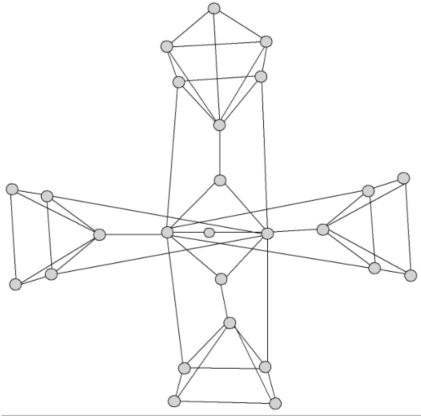
\includegraphics[width=.9\textwidth]{img/2_B11}
\end{figure}

\paragraph{B12} Niech G będzie grafem dwudzielnym o dwupodziale $(X, Y )$, gdzie $|X| = |Y |$. Przypuśćmy, że dla pewnego podzbioru $W$ zbioru $X$ mamy $|N(W)| < |W|$, tzn. graf $G$ nie spełnia warunku Halla, a zatem nie ma skojarzenia doskonałego. Znajdź w $G$ zbiór $S$, który nie spełnia warunku Tutte’a.

\paragraph{B13} Poniższą planszę chcemy pokryć kostkami domina $1 \times 2$ tak, by każde pole było przykryte, a kostki nie nachodziły na siebie i nie wystawały poza planszę. Zinterpretuj problem grafowo i rozwiąż.

\begin{figure}[H]
\centering
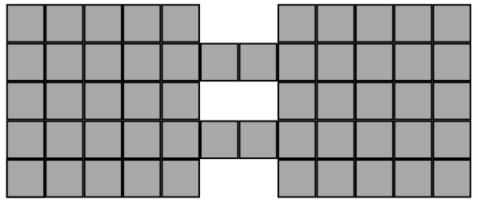
\includegraphics[width=.9\textwidth]{img/2_B13}
\end{figure}


\subsection{Zadania}
\paragraph{Zad.1} Niech $k > 1$ będzie liczbą naturalną. W pewnej grupie nieznajomych sobie pań i nieznajomych sobie panów każda pani zna przynajmniej $k$ panów, a każdy pan zna co najwyżej $k$ pań. Udowodnij, że takim grafie znajomości zawsze znajdziemy skojarzenie nasycające zbiór pań.
\paragraph{Zad.2} Uzasadnij, że każdy $k$-regularny ($k > 1$) graf dwudzielny można rozbić na $k$ rozłącznych skojarzeń doskonałych.
\paragraph{Zad.3} Dana jest macierz zero-jedynkowa $n \times m$, taka że każdy wiersz i każda kolumna zawiera dokładnie $k$ jedynek ($k > 1$). Uzasadnij, że można wybrać w tej macierzy $n$ jedynek tak, by każda kolumna i każdy wiersz zawierały tylko jedną z wybranych jedynek.
\paragraph{Zad.4}. Podaną planszę chcemy pokryć kostkami domina $1 \times 2$ tak, by każde pole było przykryte, a kostki nie nachodziły na siebie i nie wystawały poza planszę. Zinterpretuj problem grafowo i rozwiąż.
\begin{figure}[H]
\centering
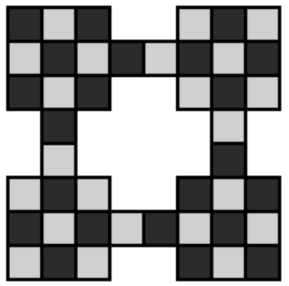
\includegraphics[width=.6\textwidth]{img/2_zad_4}
\end{figure}

\paragraph{Zad.5} Dla każdego $k > 2$ podaj przykład grafu $k$-regularnego, który nie ma skojarzenia doskonałego.

%--------------------------------------------------
\end{document}
